\documentclass[main.tex]{subfiles}

\begin{document}

\section{Motion Equation}
\label{sec:motion-equation}
Consider a variable length pendulum (VLP) as shown in Fig. \ref{vlp} and assume the following properties in order to define the equations of motion of the system

\begin{enumerate}
    \item the friction at the pivot $O$ and the viscous friction of the rod are considered absent
    \item the angle $\theta(t)$ to be between the pendulum and the vertical axis
    \item the length of the pendulum $l(t)$ that starts from the origin $O$ to the mass of the pendulum $m$
    \item the rod is considered massless
    \item  $f(t)$ is the force acting on the mass
\end{enumerate}
\begin{figure}[H]
    \centering
    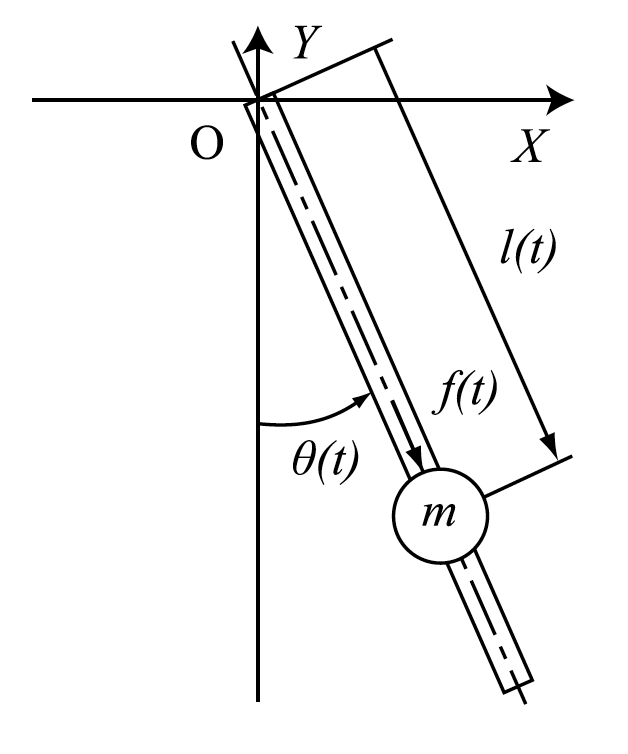
\includegraphics[scale = 0.5]{figures/pendulum.png}
    \caption{Variable Length Pendulum \cite{xin2014control}}
    \label{vlp}
\end{figure}
Since the rod is massless, the position coordinates $(x_G,y_G)$
of the COM of the VLP is defined such that
\begin{eqnarray}
x_G = l(t)\sin\theta(t) &  y_G = -l(t)\cos\theta(t) 
\end{eqnarray}
The kinetic energy $T$ of the VLP is defined as
\begin{equation}
    T = \frac{1}{2}m(\dot{x}_G^2+\dot{y}_G^2) = \frac{1}{2}m\big(l(t)\dot{\theta}(t)\big)^2+\frac{1}{2}m\big(\dot{l}(t)\big)^2 
\end{equation}
while the potential energy as
\begin{equation}
    P = mgy_G = -mgl(t)\cos\theta(t)  
\end{equation}
Using the kinetic and the potential energy, the Lagrangian equation of the VLP can be defined as
\begin{equation*}
    L = T-P
\end{equation*}
Applying the Euler-Lagrangian operator on the defined Lagrangian equation $L$, where the Lagrangian operator is given as
\begin{equation}\label{model}
\frac{\partial L}{\partial q}   -\frac{dL}{dt}\Bigg(\frac{\partial L}{\partial \dot{q}}\Bigg) = \tau
\end{equation}
with $q = [l, \theta]^T$ state vector and $\tau$ applied generalized forces on the VLP, it is possible to obtain the
equations of motions of the system
\begin{align} \label{full_model}
&\Ddot{\theta}(t)+\frac{2\dot{l}(t)\dot{\theta}(t)}{l(t)} + \frac{g\sin\theta(t)}{l(t)} = 0  \\
\label{second_model}
&\Ddot{l}(t)-ml(t)\dot{\theta}^2(t)-mg\cos\theta(t) = f(t)
\end{align}
For simplicity, the control input will be chosen to be $$u =\Ddot{l}(t)$$
where $f(t)$ can be computed directly from equation \eqref{second_model}.

\section{Problem Formulation}
\label{sec:problem-formulation}
The total mechanical energy of the system can be expressed as the sum of the kinetic and the potential energy
\begin{equation} \label{total_energy}
    E_T = T+P = \frac{1}{2}\dot{l}^2(t)+\frac{1}{2}\big(l(t)\dot{\theta}(t)\big)^2-gl(t)\cos\theta(t) 
 \end{equation}
where, without loss of generality, it is assumed that $m = 1$. 
%\paragraph{}
Consider the desired trajectory of swing to be described by
\begin{equation}
    E_r = \frac{1}{2}\big(l_r\dot{\theta}(t)\big)^2-gl_r\cos\theta(t) 
\end{equation}
where, for a given desired length of the pendulum $l_r$ and a maximal angle $\theta_{max}$ of desired swing. $E_r$ is the 
desired energy, which satisfies the following
\begin{eqnarray}
  \label{eq:Er-property}
 E_r = -gl_r\cos\theta_{max}, & \hfill &\theta_{max} \in (0,\pi]
\end{eqnarray}
 The trajectory tracking problem proposed in \cite{xin2014control} is to design a control law $u$ in order to achieve the following
 \begin{eqnarray} \label{control_obj}
  \lim_{t\rightarrow \infty} E_T = E_r  \ \ \ \ \ \  \lim_{t\rightarrow \infty} \dot{l} = 0 \ \ \ \ \ \  \ \ \lim_{t\rightarrow \infty} l = l_r
 \end{eqnarray}

\end{document}